%%%%%%%%%%%%%%%%%%%%%%%%%%%%%%%%%%%%%%%%%
% Beamer Presentation
% LaTeX Template
% Version 1.0 (10/11/12)
%
% This template has been downloaded from:
% http://www.LaTeXTemplates.com
%
% License:
% CC BY-NC-SA 3.0 (http://creativecommons.org/licenses/by-nc-sa/3.0/)
%
%%%%%%%%%%%%%%%%%%%%%%%%%%%%%%%%%%%%%%%%%

%----------------------------------------------------------------------------------------
%	PACKAGES AND THEMES
%----------------------------------------------------------------------------------------

\documentclass{beamer}
\usepackage{xcolor}
\usepackage{graphicx}
\usepackage{tikz}
\usepackage{listings}
\usepackage{multicol}

\definecolor{applegreen}{rgb}{0.55, 0.71, 0.0}
\definecolor{blue(ncs)}{rgb}{0.0, 0.45, 0.60}
\definecolor{burgundy}{rgb}{0.5, 0.0, 0.13}

\lstdefinestyle{qfunc}{
  language=C,
  emptylines=1,
  breaklines=true,
  basicstyle=\ttfamily\color{black},
  moredelim=**[is][\color{applegreen}]{@}{@},
  moredelim=**[is][\color{blue(ncs)}]{!}{!},
  moredelim=**[is][\color{applegreen!40!black}]{<}{<},
  moredelim=**[is][\color{blue(ncs)!80}]{#}{#},
  moredelim=**[is][\color{blue(ncs)!80!black}]{'}{'},
}

\lstdefinestyle{oper}{
  language=C,
  emptylines=1,
  breaklines=true,
  basicstyle=\ttfamily\color{black},
  moredelim=**[is][\color{applegreen}]{@}{@},
  moredelim=**[is][\color{blue(ncs)}]{!}{!},
  moredelim=**[is][\color{burgundy}]{#}{#},
  moredelim=**[is][\color{red}]{'}{'},
  moredelim=**[is][\bf]{<}{<},
}

\mode<presentation> {

\usetheme{CambridgeUS}

\usecolortheme{wolverine}

\definecolor{gold}{HTML}{D4A017}
\definecolor{darkgold}{HTML}{B7950B}

\setbeamercolor{palette primary}{bg=gold,fg=white}
\setbeamercolor{palette secondary}{bg=darkgold,fg=white}
\setbeamercolor{palette tertiary}{bg=black,fg=white}
\setbeamercolor{palette quaternary}{bg=gold,fg=white}

\setbeamercolor{frametitle}{bg=darkgold,fg=white}

\setbeamercolor{section number projected}{bg=black,fg=gold}
\setbeamercolor{item}{fg=black,bg=gold}

\setbeamertemplate{page number in head/foot}[framenumber]
}

\usepackage{graphicx} % Allows including images
\usepackage{booktabs} % Allows the use of \toprule, \midrule and \bottomrule in tables

%----------------------------------------------------------------------------------------
%	TITLE PAGE
%----------------------------------------------------------------------------------------

\title[libCEED Finite Element Library]{Matrix Free P-Multigrid with libCEED and PETSc} % The short title appears at the bottom of every slide, the full title is only on the title page

\author{Jeremy L Thompson} % Your name
\institute[CU Boulder] % Your institution as it will appear on the bottom of every slide, may be shorthand to save space
{University of Colorado Boulder \\ % Your institution for the title page
\medskip
\textit{jeremy.thompson@colorado.edu} % Your email address
}
\date{June 28, 2019} % Date, can be changed to a custom date

\begin{document}

\begin{frame}
\titlepage % Print the title page as the first slide
\end{frame}

%------------------------------------------------

\begin{frame}
\begin{center}
\frametitle{libCEED Team}

{\flushleft

Developers: \hspace{2mm} Jed Brown\textsuperscript{1}, Jeremy Thompson\textsuperscript{1} \\
\hspace{23mm} Valeria Barra\textsuperscript{1}, Tzanio Kolev\textsuperscript{2}, Jean-Sylvain Camier\textsuperscript{2},\\
\hspace{23mm} Veselin Dobrev\textsuperscript{2}, Yohann Doudouit\textsuperscript{2}, Tim Warburton\textsuperscript{3},\\
\hspace{23mm} David Medina\textsuperscript{4}, \& Thilina Rathnayake\textsuperscript{5}\\

~\\

Grant: \hspace{11mm} Exascale Computing Project (17-SC-20-SC)\\

~\\

~\\

\small{1: University of Colorado, Boulder\\
2: Lawrence Livermore National Laboratory\\
3: Virginia Polytechnic Institute and State University\\
4: OCCA\\
5: University of Illinois, Urbana-Champaign\\}}

\end{center}
\end{frame}

\begin{frame}
\begin{center}
\frametitle{Overview}

libCEED is an extensible library that provides a portable algebraic\\interface and optimized implementations of high-order operators\\

~\\

We have optimized implementations targeting CPU and GPU\\

~\\

We investigate a p-multigrid example with PETSc PCMG

\end{center}
\end{frame}
 
%------------------------------------------------

\begin{frame}
\frametitle{Overview} % Table of contents slide, comment this block out to remove it
\tableofcontents % Throughout your presentation, if you choose to use \section{} and \subsection{} commands, these will automatically be printed on this slide as an overview of your presentation
\end{frame}

%----------------------------------------------------------------------------------------
%	PRESENTATION SLIDES
%----------------------------------------------------------------------------------------

%------------------------------------------------
\section{Introduction}
%------------------------------------------------

\begin{frame}
\begin{center}
\frametitle{Center for Efficient Exascale Discretizations}

\begin{flushleft}
DoE exascale co-design center\\

~\\
\end{flushleft}

\begin{itemize}

\item Design discretization algorithms for exascale hardware that deliver significant performance gain over low order methods\\

~\\

\item Collaborate with hardware vendors and software projects for exascale hardware and software stack\\

~\\

\item Provide efficient and user-friendly unstructured PDE discretization component for exascale software ecosystem

\end{itemize}

\end{center}
\end{frame}

%------------------------------------------------

\begin{frame}
\begin{center}
\frametitle{Matrix Free}

libCEED design approach:\\

~\\

\begin{itemize}

\item Avoid global matrix assembly\\

~\\

\item Map each element to reference element\\

~\\

\item Geometry data computed on the fly or precomputed\\

~\\

\item Easy to parallelize across hetrogeneous nodes

\end{itemize}

\end{center}
\end{frame}

%------------------------------------------------

\begin{frame}
\begin{center}
\frametitle{libCEED}

libCEED provides multiple backend implementations\\

~\\

\begin{itemize}

\item CPU

\begin{itemize}

\item Pure C

\item Advanced Vector Instructions

\item LIBXSMM

\end{itemize}

~\\

\item GPU

\begin{itemize}

\item Pure CUDA

\item OCCA

\item MAGMA

\end{itemize}

\end{itemize}

\end{center}
\end{frame}

%------------------------------------------------

\begin{frame}
\begin{center}
\frametitle{libCEED}

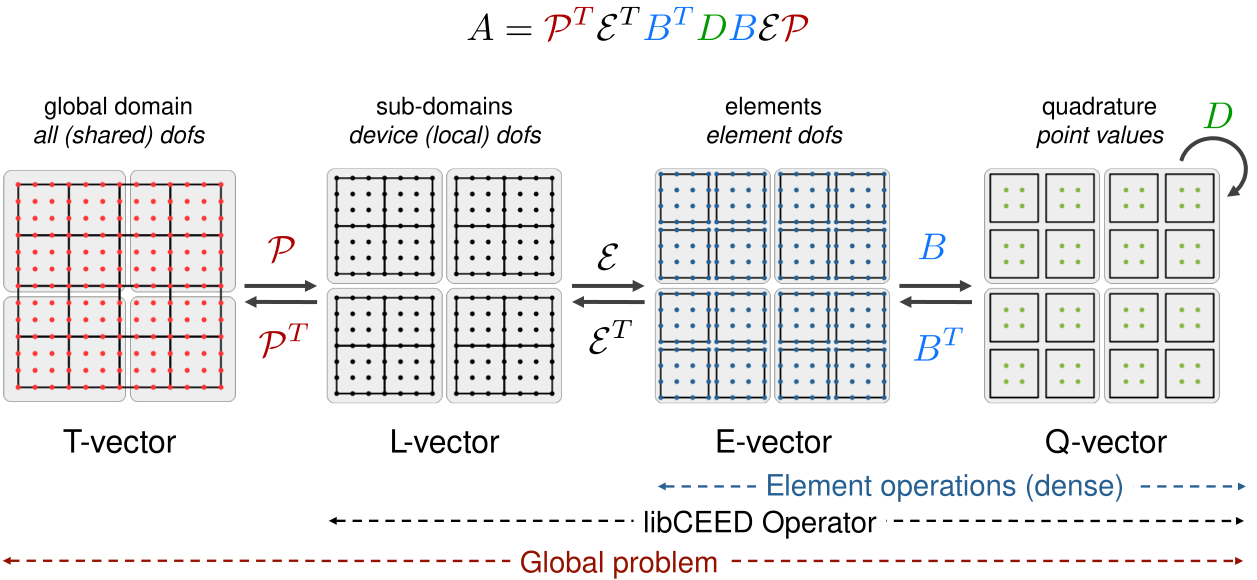
\includegraphics[height=4.5cm]{libCEEDAPI}

\small{

\hspace{1.8cm}${\color{burgundy}A}_L = G^T {\color{blue(ncs)}B^T} {\color{applegreen}D} {\color{blue(ncs)}B} G$

\begin{itemize}

\item $G$ - CeedElemRestriction, local gather/scatter

\item {\color{blue(ncs)}$B$} - CeedBasis, provides basis operations such as interp and grad

\item {\color{applegreen}$D$} - CeedQFunction, representation of PDE at quadrature points

\item ${\color{burgundy}A}_L$ - CeedOperator, aggregation of Ceed objects for local action of operator

\end{itemize}

}

\end{center}
\end{frame}

%------------------------------------------------
\section{Multigrid Example}
%------------------------------------------------

\begin{frame}
\begin{center}
\frametitle{PETSc PCMG}

\begin{itemize}

\item PCMG - PETSc geometric multigrid preconditioner\\

~\\

\item Requires several operators from the user\\

~\\

\begin{itemize}

\item Restriction operator\\

~\\

\item Interpolation operator\\

~\\

\item Smoother\\

~\\

\item Coarse grid solver

\end{itemize}

\end{itemize}

\end{center}
\end{frame}

%------------------------------------------------

\begin{frame}
\begin{center}
\frametitle{PETSc PCMG}

3 level multigrid with PCMG\\
~\\

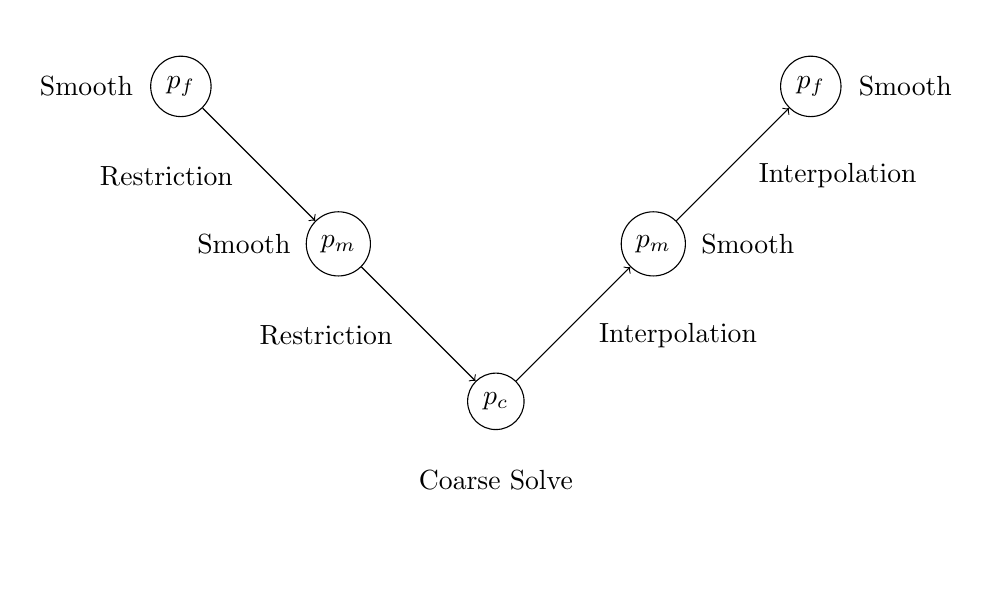
\begin{tikzpicture}
\node[shape=circle,draw=black] (A) at (0,0) {$p_f$};
\node[shape=circle] (Al) at (-1.2,0) {Smooth};
\node[shape=circle,draw=black] (B) at (2,-2) {$p_m$};
\node[shape=circle] (Bl) at (0.8,-2) {Smooth};
\node[shape=circle,draw=black] (C) at (4,-4) {$p_c$};
\node[shape=circle] (Cl) at (4,-5) {Coarse Solve};
\node[shape=circle,draw=black] (D) at (6,-2) {$p_m$};
\node[shape=circle] (Dl) at (7.2,-2) {Smooth};
\node[shape=circle,draw=black] (E) at (8,0) {$p_f$};
\node[shape=circle] (El) at (9.2,0) {Smooth};
\path[->] (A) edge node[left=10, pos=.6] {Restriction} (B);
\path[->] (B) edge node[left=10, pos=.6] {Restriction} (C);
\path[->] (C) edge node[right=10, pos=.4] {Interpolation} (D);
\path[->] (D) edge node[right=10, pos=.4] {Interpolation} (E);
\end{tikzpicture}

\end{center}
\end{frame}

%------------------------------------------------

\begin{frame}
\begin{center}
\frametitle{libCEED Operators - Diffusion}

Solving the 2D Poisson problem: $-\Delta u = f$\\

Weak Form: $\int \nabla v \nabla u = \int v f$\\
~\\

\begin{itemize}

\item General libCEED Operator

${\color{burgundy}A}_L = G^T {\color{blue(ncs)}B^T} {\color{applegreen}D} {\color{blue(ncs)}B} G$\\
~\\

\item Diffusion Operator

${\color{burgundy}A}_L = G^T {\color{blue(ncs)}\hat{D}_{2d}^T} {\color{applegreen}D} {\color{blue(ncs)}\hat{D}_{2d}} G$

\end{itemize}

where ${\color{applegreen}D}$ is block diagonal by quadrature point:\\
${\color{applegreen}D_i} = \left( w_i \det{J_{geo}}\right) J_{geo}^{-T} J_{geo}^{-1}$ and
$J_{geo} = \left[ \begin{tabular}{cc}
$\frac{\partial x}{\partial r}$ & $\frac{\partial x}{\partial s}$\\
$\frac{\partial y}{\partial r}$ & $\frac{\partial y}{\partial s}$
\end{tabular} \right]$

\end{center}
\end{frame}

%------------------------------------------------

\begin{frame}
\begin{center}
\frametitle{libCEED Operators - Diffusion}

Solving the 2D Poisson problem: $-\Delta u = f$\\

Weak Form: $\int \nabla v \nabla u = \int v f$\\
~\\

\begin{itemize}

\item General libCEED Operator

${\color{burgundy}A}_L = G^T {\color{blue(ncs)}B^T} {\color{applegreen}D} {\color{blue(ncs)}B} G$\\
~\\

\item Diffusion Operator

${\color{burgundy}A}_L = G^T {\color{blue(ncs)}\hat{D}_{2d}^T} {\color{applegreen}D} {\color{blue(ncs)}\hat{D}_{2d}} G$\\
~\\

\item Computationaly Efficient Form

${\color{burgundy}A}_L = G^T {\color{blue(ncs)} \left[ \begin{tabular}{cc}
$\hat{D}^T \otimes \hat{J}^T$ & $\hat{J}^T \otimes \hat{D}^T$
\end{tabular} \right]} {\color{applegreen}D} {\color{blue(ncs)} \left[ \begin{tabular}{c}
$\hat{D} \otimes \hat{J}$\\
$\hat{J} \otimes \hat{D}$
\end{tabular} \right]} {\color{black} G}$\\

\end{itemize}

\end{center}
\end{frame}

%------------------------------------------------

\begin{frame}
\begin{center}
\frametitle{libCEED Operators - Diffusion}

Solving the 2D Poisson problem: $-\Delta u = f$\\

Weak Form: $\int \nabla v \nabla u = \int v f$\\
~\\

\begin{itemize}

\item General libCEED Operator

${\color{burgundy}A}_L = G^T {\color{blue(ncs)}B^T} {\color{applegreen}D} {\color{blue(ncs)}B} G$\\
~\\

\item Diffusion Operator

${\color{burgundy}A}_L = G^T {\color{blue(ncs)}\hat{D}_{2d}^T} {\color{applegreen}D} {\color{blue(ncs)}\hat{D}_{2d}} G$\\
~\\

\item Computationaly Efficient Form

${\color{burgundy}A}_L = G^T {\color{blue(ncs)} \left( \hat{J}^T \otimes \hat{J}^T \right) \left[ \begin{tabular}{cc}
$\tilde{D}^T \otimes I$ & $I \otimes \tilde{D}^T$
\end{tabular} \right]} {\color{applegreen}D} {\color{blue(ncs)} \left[ \begin{tabular}{c}
$\tilde{D} \otimes I$\\
$I \otimes \tilde{D}$
\end{tabular} \right] \left( \hat{J} \otimes \hat{J} \right)} {\color{black} G}$\\
where ${\color{blue(ncs)}\hat{D} = \tilde{D} \hat{J}}$

\end{itemize}

\end{center}
\end{frame}

%------------------------------------------------

\begin{frame}
\begin{center}
\frametitle{libCEED Operators - Restriction}

Restriction / Interpolation is largely a basis operation\\
~\\

\begin{itemize}

\item General libCEED Operator

${\color{burgundy}A}_L = G^T {\color{blue(ncs)}B^T} {\color{applegreen}D} {\color{blue(ncs)}B} G$\\
~\\

\item Restriction / Interpolation Operator

${\color{burgundy}A}_L = G_c^T {\color{blue(ncs)}I} {\color{applegreen}I} {\color{blue(ncs)}B_{f to c}} G_f$\\
~\\

\item Computationaly Efficient Form

${\color{burgundy}A}_L = G_c^T {\color{blue(ncs)}\left( \hat{J}_{f to c} \otimes \hat{J}_{f to c} \right)} G_f$

\end{itemize}

\end{center}
\end{frame}

%------------------------------------------------

\begin{frame}
\begin{center}
\frametitle{libCEED Operators - Smoothing}

For smoothing, we use a libCEED diffusion operator\\with KSPCHEBYCHEV\\
~\\

\begin{itemize}

\item General libCEED Operator

${\color{burgundy}A}_L = G^T {\color{blue(ncs)}B^T} {\color{applegreen}D} {\color{blue(ncs)}B} G$\\
~\\

\item Diffusion Operator

${\color{burgundy}A}_L = G^T {\color{blue(ncs)}\hat{D}_{2d}^T} {\color{applegreen}D} {\color{blue(ncs)}\hat{D}_{2d}} G$\\
~\\

\item Computationaly Efficient Form

${\color{burgundy}A}_L = G^T {\color{blue(ncs)} \left( \hat{J}^T \otimes \hat{J}^T \right) \left[ \begin{tabular}{cc}
$\tilde{D}^T \otimes I$ & $I \otimes \tilde{D}^T$
\end{tabular} \right]} {\color{applegreen}D} {\color{blue(ncs)} \left[ \begin{tabular}{c}
$\tilde{D} \otimes I$\\
$I \otimes \tilde{D}$
\end{tabular} \right] \left( \hat{J} \otimes \hat{J} \right)} {\color{black} G}$

\end{itemize}

\end{center}
\end{frame}

%------------------------------------------------

\begin{frame}[fragile]
\begin{center}
\frametitle{QFunction Definition}

General libCEED QFunction:\\

${\color{blue(ncs)!80!black}v_q} = {\color{applegreen}D} {\color{blue(ncs)!80}u_q}$\\

~\\

2D Diffusion QFunction:\\

${\color{blue(ncs)}\left[} {\color{blue(ncs)!80!black} \begin{tabular}{c}
$v_1$\\ $v_2$ \end{tabular}} {\color{blue(ncs)}\right]} = {\color{applegreen} \left[} {\color{green!40!black} \begin{tabular}{cc}
$D_{00}$ & $D_{01}$\\
$D_{01}$ & $ D_{11}$ \end{tabular}} {\color{applegreen}\right]} {\color{blue(ncs)}\left[} {\color{blue(ncs)!80} \begin{tabular}{c}
$u_1$\\ $u_2$ \end{tabular} } {\color{blue(ncs)}\right]}$\\

~\\~\\

Code:
{\scriptsize
\begin{lstlisting}[style=qfunc]
CeedQFunctionCreateInterior(ceed, 1, Diff,
                            __FILE__multigrid.c:Diff, &@qf_apply@);
CeedQFunctionAddInput(@qf_apply@, #"u"#, 1, !CEED_EVAL_GRAD!);
CeedQFunctionAddInput(@qf_apply@, <"geo"<, 3, CEED_EVAL_NONE);
CeedQFunctionAddOutput(@qf_apply@, '"v"', 1, !CEED_EVAL_GRAD!);
\end{lstlisting}
}

\end{center}
\end{frame}

%------------------------------------------------

\begin{frame}[fragile]
\begin{center}
\frametitle{Operator Definition}

General libCEED Operator:\\

${\color{red}v}_L = {\color{burgundy}A}_L {\color{red}u}_L$\\

~\\

2D Diffusion Operator:\\

${\color{burgundy}A}_L = {\bf G^T} {\color{blue(ncs)}B^T} {\color{applegreen}D} {\color{blue(ncs)}B} {\bf G}$\\

~\\~\\

Code:
{\scriptsize
\begin{lstlisting}[style=oper]
CeedOperatorCreate(ceed, @qf_apply@, NULL, NULL, &#op_apply#);
CeedOperatorSetField(#op_apply#, "u", <Erestrictu<, CEED_TRANSPOSE,
                     !basisu!, 'CEED_VECTOR_ACTIVE');
CeedOperatorSetField(#op_apply#, "geo",Erestrictqdi,CEED_NOTRANSPOSE,
                     !CEED_BASIS_COLLOCATED!, geo);
CeedOperatorSetField(#op_apply#, "v", <Erestrictu<, CEED_TRANSPOSE,
                     !basisu!, 'CEED_VECTOR_ACTIVE');
...
CeedOperatorApply(#op_apply#, 'xloc', 'yloc', CEED_REQUEST_IMMEDIATE);
\end{lstlisting}
}

\end{center}
\end{frame}

%------------------------------------------------

\begin{frame}
\begin{center}
\frametitle{Performance}

\begin{itemize}

\item $3$D Poisson Problem\\

~\\

\item Test run on personal computer\\

~\\

\item Mesh

\begin{itemize}

\item $8^3$ GLL points per element

\item Quadrature on $9^3$ GL points per element

\item Cube with $30$ elements, $11,880$ DoFs

\end{itemize}

\end{itemize}

{\small

\setlength\columnsep{1pt}

\begin{multicols}{2}

\begin{itemize}

\setlength{\leftmarginii}{1em}

\item Unpreconditioned

\begin{itemize}

\item 5.0057e-07 \hfill $\lvert \lvert \cdot \rvert \rvert_\infty$ Error \hspace{1em}

\item $119$ \hfill CG iterations \hspace{1em}

\item 0.2148 million \hfill CG DoFs/sec \hspace{1em}

\item 13.5436 sec \hfill CG solve time \hspace{1em}

\end{itemize}

\item P-Multigrid

\begin{itemize}

\item 5.0059e-07 \hfill $\lvert \lvert \cdot \rvert \rvert_\infty$ Error \hspace{1em}

\item $18$ \hfill CG iterations \hspace{1em}

\item 0.0795 million \hfill CG DoFs/sec \hspace{1em}

\item 4.1058 sec \hfill CG solve time \hspace{1em}

\end{itemize}

\end{itemize}

\end{multicols}

}

\end{center}
\end{frame}

%------------------------------------------------

\begin{frame}
\begin{center}
\frametitle{Performance - Highlights}

\begin{itemize}

\item Significantly decreased number of iterations\\

~\\

\item Iterations slower than expected\\

~\\

\item Want to decrease iteration time with lighter preconditioner\\

~\\

\item Caveats:

\begin{itemize}

\item Small mesh run on laptop for demo purposes\\

~\\

\item Need minor PETSc code adjustments to run well on GPU

\end{itemize}

\end{itemize}

\end{center}
\end{frame}

%------------------------------------------------
\section{Future Work}
%------------------------------------------------

\begin{frame}
\begin{center}
\frametitle{Future Work}

\begin{itemize}

\item Further performance tuning (GPU and CPU)\\

~\\

\item Unstructured mesh examples (with AMG coarse solve)\\

~\\

\item Expanded set of non-linear examples\\

~\\

\item Preconditioning based on libCEED operator decomposition\\

~\\

\item Efficient diagonal computation for preconditioning\\

~\\

\item Algorithmic differentiation of user quadrature functions\\

~\\

\item We invite contributors and friendly users

\end{itemize}

\end{center}
\end{frame}

%------------------------------------------------
\section{Questions}
%------------------------------------------------

\begin{frame}
\begin{center}
\frametitle{Questions?}

{\flushleft

Advisors : \hspace{5mm} Jed Brown\textsuperscript{1} \& Daniel Appel\"{o}\textsuperscript{1}\\

~\\

Collaborators: Valeria Barra\textsuperscript{1}, Oana Marin\textsuperscript{2}, Tzanio Kolev\textsuperscript{3},\\
\hspace{23mm} Jean-Sylvain Camier\textsuperscript{3}, Veselin Dobrev\textsuperscript{3}, Yohann Doudouit\textsuperscript{3},\\
\hspace{23mm} Tim Warburton\textsuperscript{4}, David Medina\textsuperscript{5}, \& Thilina Rathnayake\textsuperscript{6}\\

~\\

Grant: \hspace{11mm} Exascale Computing Project (17-SC-20-SC)\\

~\\

~\\

\small{1: University of Colorado, Boulder\\
2: Argonne National Laboratory\\
3: Lawrence Livermore National Laboratory\\
4: Virginia Polytechnic Institute and State University\\
5: OCCA\\
6: University of Illinois, Urbana-Champaign\\}}

\end{center}
\end{frame}

%------------------------------------------------

\begin{frame}[noframenumbering]
\titlepage % Print the title page
\end{frame}

%------------------------------------------------

%----------------------------------------------------------------------------------------

\end{document}

